% ОБЯЗАТЕЛЬНО ИМЕННО ТАКОЙ documentclass!
% (Основной кегль = 14pt, поэтому необходим extsizes)
% Формат, разумеется, А4
% article потому что стандарт не подразумевает разделов
% Глава = section, Параграф = subsection
% (понятия "глава" и "параграф" из документа, описывающего диплом)
\documentclass[a4paper,article,14pt]{extarticle}

% Подключаем главный пакет со всем необходимым
\usepackage{spbudiploma_tempora}


% Пакеты по желанию (самые распространенные)
% Хитрые мат. символы
\usepackage{euscript}
% Таблицы
\usepackage{longtable}
\usepackage{makecell}
% Картинки (можно вставлять даже pdf)
\usepackage[pdftex]{graphicx}
\usepackage{graphicx}
\usepackage{subfig}
\usepackage{amsthm,amssymb, amsmath}
\usepackage{textcomp}
\usepackage{listings}

\usepackage{xcolor}

\definecolor{comments_color}{RGB}{140, 140, 140}
\definecolor{key_words_color}{RGB}{0, 51, 179}

\lstset{
    language=Python,        % Язык кода
    basicstyle=\small,   % Основной стиль
    keywordstyle=\color{key_words_color},  % Стиль для ключевых слов
    commentstyle=\color{comments_color}, % Стиль для комментариев
    stringstyle=\color{red},    % Стиль для строк
    numbers=left,          % Нумерация строк слева
    numberstyle=\tiny\color{gray}, % Стиль для номеров строк
    stepnumber=1,          % Нумеровать каждую строку
    numbersep=5pt,         % Отступ номеров строк
    % backgroundcolor=\color{lightgray}, % Цвет фона
    showspaces=false,      % Не показывать пробелы
    showstringspaces=false % Не показывать пробелы в строках
}


\begin{document}

% Титульник в файле titlepage.tex
% --------------------- Титульник ВКР СПбГУ -----------------------------
% Автор: Тоскин Николай, itonik@me.com
% Если заметили ошибку, напишите на email
% Если хотите добавить изменение самостоятельно:
% https://github.com/itonik/spbu_diploma/
% Использованы материалы:
% habr.com/ru/post/144648/
% cpsconf.ru
% Документы ниже могут уже быть неактуальны, тем не менее за годы ничего
% нового не появилось
% Текст:
% http://edu.spbu.ru/images/data/normativ_acts/local/20181030_10432_1.pdf
% Титульный лист:
% http://edu.spbu.ru/images/data/normativ_acts/local/20180703_6616_1.pdf
% -----------------------------------------------------------------------

% Титульный лист диплома СПбГУ
% Временное удаление foot на titlepage
\newgeometry{left=30mm, top=20mm, right=15mm, bottom=20mm, nohead, nofoot}
\begin{titlepage}
\begin{center}

\textbf{Санкт--Петербургский}
\textbf{государственный университет}

\vspace{35mm}

\textbf{\textit{\large Нечаев Илья Андреевич}} \\[8mm]
% Название
\textbf{\large Выпускная квалификационная работа}\\[3mm]
\textbf{\textit{\large Разработка бортового измерительного комплекса для ледокола}}

\vspace{20mm}
Уровень образования: бакалавриат\\
Направление 02.03.01 «Математика и компьютерные науки»\\
Основная образовательная программа СВ.5152 «Математика, алгоритмы и
анализ данных»\\
Профиль «Науки о данных»\\[25mm]


% Научный руководитель, рецензент
\begin{flushright}
\begin{minipage}[t]{0.65\textwidth}
{Научный руководитель:} \\
доцент,
факультет математики \\
и компьютерных наук СПбГУ,
к.ф. --- м.н., \\
Шалымов Дмитрий Сергеевич

\vspace{10mm}

{Рецензент:} \\
Главный инженер по разработке, \\ОАО СберАвтоТех \\ Булаев Владимир Владимирович
\end{minipage}
\end{flushright}

\vfill 

{Санкт-Петербург}
\par{\the\year{} г.}
\end{center}
\end{titlepage}
% Возвращаем настройки geometry обратно (то, что объявлено в преамбуле)
\restoregeometry{}
% Добавляем 1 к счетчику страниц ПОСЛЕ titlepage, чтобы исключить 
% влияние titlepage environment
\addtocounter{page}{1}

% Содержание
\tableofcontents
\pagebreak

\section{Введение}
\begin{figure}[htbp]
    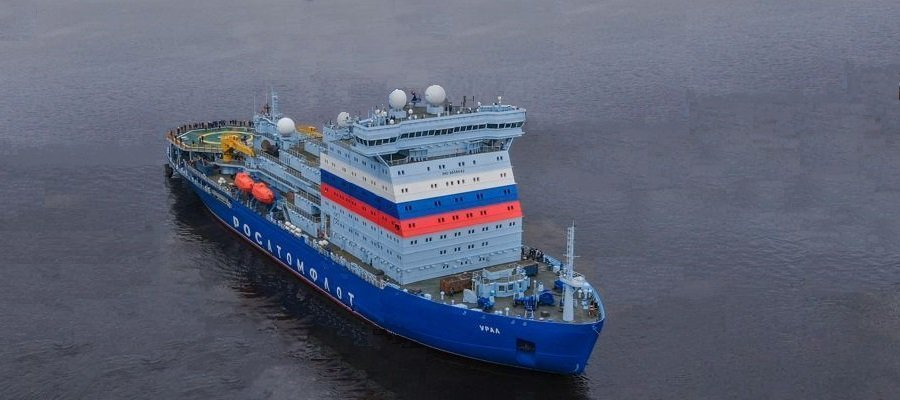
\includegraphics[scale=0.5]{src/Introduction/assets/Ледокол.jpg}
\caption{Ледокол Урал}\label{fig:IceBreker}
\end{figure}
Развитие судоходства в Арктике требует создания и внедрения современных технологических решений для обеспечения безопасности и 
эффективности морских операций. Ледоколы играют ключевую роль в освоении этих регионов, обеспечивая проход судов через ледовые поля и выполняя различные 
научно-исследовательские и промышленные задачи. Бортовой измерительный комплекс (БИК) должен стать важной частью ледокола, поскольку позволит автоматизировать часть работы
команды судна, что позволит исследователям больше заниматься анализом данных, нежели их сбором.

Сейчас анализ ледовой обстановки выполняется человеком. Специалисту приходится при помощи камер выглядывать за борт судна, чтобы оценить толщину ледового
покрытия, самостоятельно наблюдать за эволюцией ледового канала, который оставляет за собой ледокол. БИК призван  исправить эту ситуацию, 
автоматизировав сбор информации о ледовой обстановке около ледокола.

Комплекс, разработка части которого была положена в основу данной работы, в течение зимы 2023--2024 годов и весны 2024 года был установлен на борту ледокола Урал и
тестировался всё это время.

В настоящей работе описаны результаты разработки алгоритмов для обработки изображения ледового канала. Была проанализирована литература и рассмотрены
различные подходы. Результатом работы стали два алгоритма по построению масок. Первый основан на EM алгоритме для попиксельной сегментации, он был разработан в очень сжатые сроки,
чтобы как можно раньше начать собирать данные. Второй алгоритм уже использует нейросетевой подход, основанный на бэкбоуне, обучавшемся на задаче решения пазлов, и дополненный 
предобученным трансформером с архитектурой DINO для уточнения меток. В работе представлены как описания этих алгоритмов, так и полученные результаты. 
\section{Постановка задачи}
\subsection{Задача}
Задачей в проекте было создание алгоритма для наблюдением за эволюцией ледового канала. Фактически алгоритм должен выдавать ширину канала на 
некотором удалении от кормы ледокола. Из-за недостатка ресурсов, сжатых сроков и особенностей связанных с деплоем на эксплуатирующийся ледокол задача была поделена на две части:
\begin{enumerate}
    \item Реализация при помощи тех технических средств и программного обеспечения, которые уже есть на ледоколе
    \item Реализация более точного алгоритма с возможностью использовать дополнительное программное обеспечение и, возможно, дополнительные технические средства.
\end{enumerate}

Было решено решать более общую задачу. Вместо ширины канала искать маску канала и уже по ней определять ширину и другие параметры.

На ледоколе были установлены следующие устрйства:
\begin{enumerate}
    \item Камера с разрешением 1920*1080
    \item Лидар Livox Avia
    \item Компьютер для расчетов (без видеокарты) 
\end{enumerate}

Для работы алгоритма было решено использовать снимки камеры, так как эффективная дальность лидара в детектировании ледовой поверхности не превышает 100 метров, 
в то время как камера способна ``видеть'' более, чем на километр. Однако у камеры есть другая проблема, ночные снимки камеры практически невозможно анализировать.

\begin{figure}[htbp]
    \centering
    \subfloat[Дневной снимок]{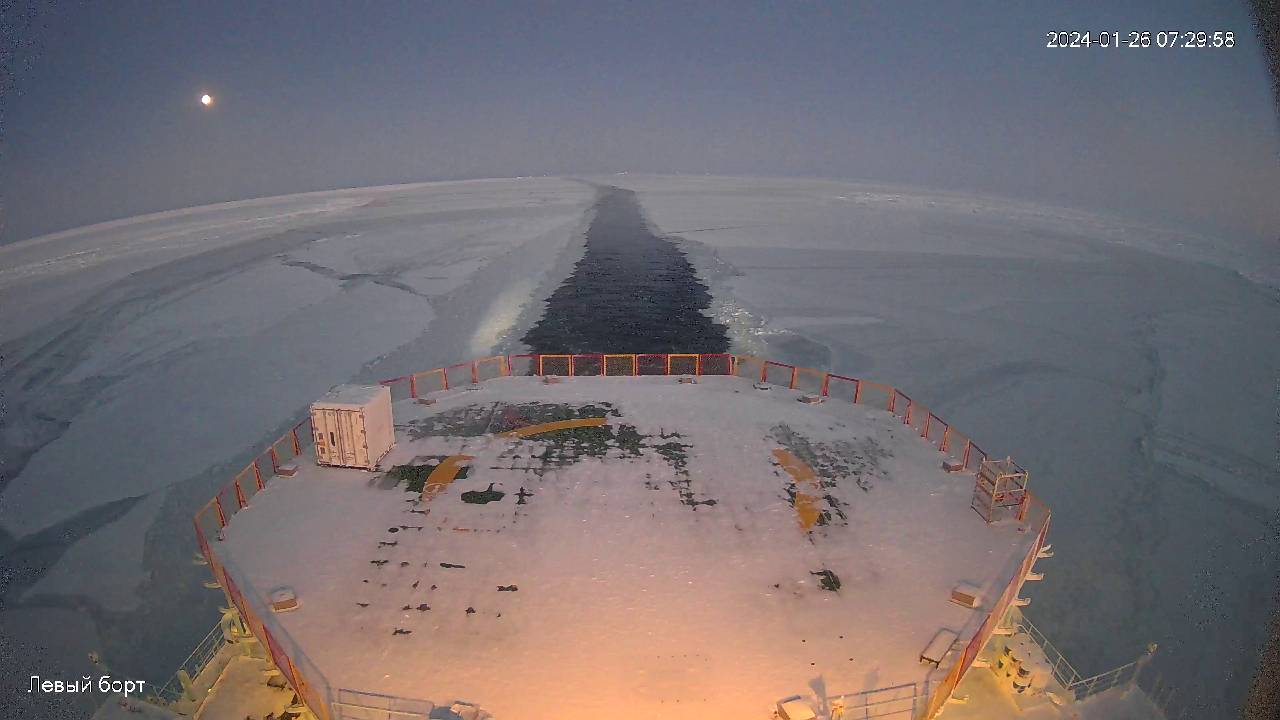
\includegraphics[scale=0.18]{src/Project_planning/assets/3920.jpg}}
    \subfloat[Ночной снимок]{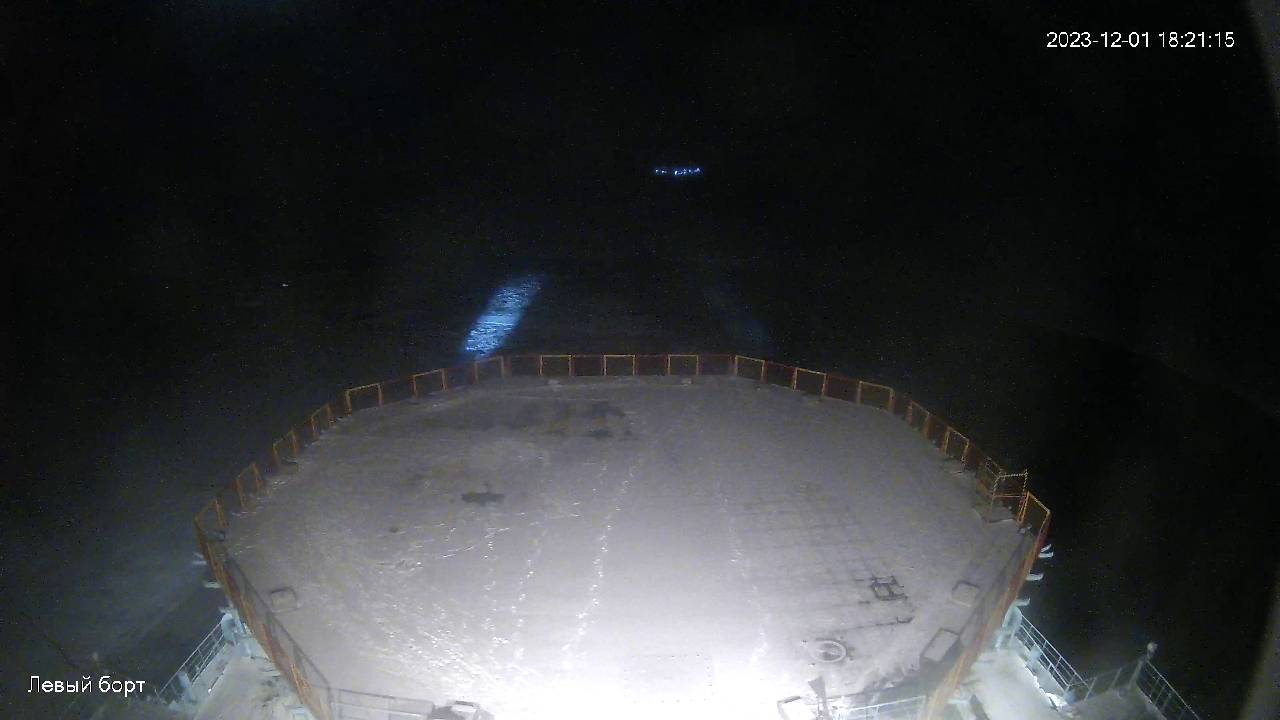
\includegraphics[scale=0.18]{src/Project_planning/assets/1145.jpg}}
    \caption{Примеры снимков кормовой камеры}\label{fig:camera_images}
\end{figure}

\subsection{Первый подход}
Поскольку в первом случае предполагалось использовать только средства уже установленные на ледокол, использовать глубокое обучение не представлялось возможным, 
так как никаких библиотек (Pytorch, TensorFlow и др) на ледоколе установлено не было. Это ставило ограничения на то, что первоначальный подход должен был 
использовать алгоритмы классического машинного обучения, а также техники компьютерного зрения, не использующие глубокое обучение.

Однако данный подход не ставил целью получения идеальной маски, так как был временным. Главной задачей первоначального подхода была разработка алгоритма, который 
мог бы выдавать маску канала, возможно сильно зашумленную, при ярком дневном освещении и при наличии в канале открытой воды.

\subsection{Второй подход}
Второй подход подразумевал возможность добавления на ледокол дополнительных библиотек, таких как Pytorch. Также ожидалось, что в комплекс помимо камеры, 
возможно будет включить тепловизор, что могло бы сильно облегчить задачу и сделать возможным наблюдение канала в ночное время суток, что особенно актуально зимой 
- в полярную ночь. Однако тепловизор так и не получилось включить в комплекс, из-за чего во второй части проекта всё также используется камера, но сам алгоритм 
уже реализован с использованием глубокого обучения.

Целью второго подхода, было создание алгоритма, способного выделять ледовый канал уже при более плохой видимости (в сумерках, в тумане, во время снегопада и т.д.), 
а также способный выделять ледовый канал покрытый ледяным салом (снегом и упавшим в него льдом). Данный подход уже не был скован узкими временными рамками, так как 
его установка на ледокол ожидается летом 2024 года.

\subsection{Общие ограничения}
\begin{figure}[htbp]
    \centering
    \subfloat[Заросший канал]{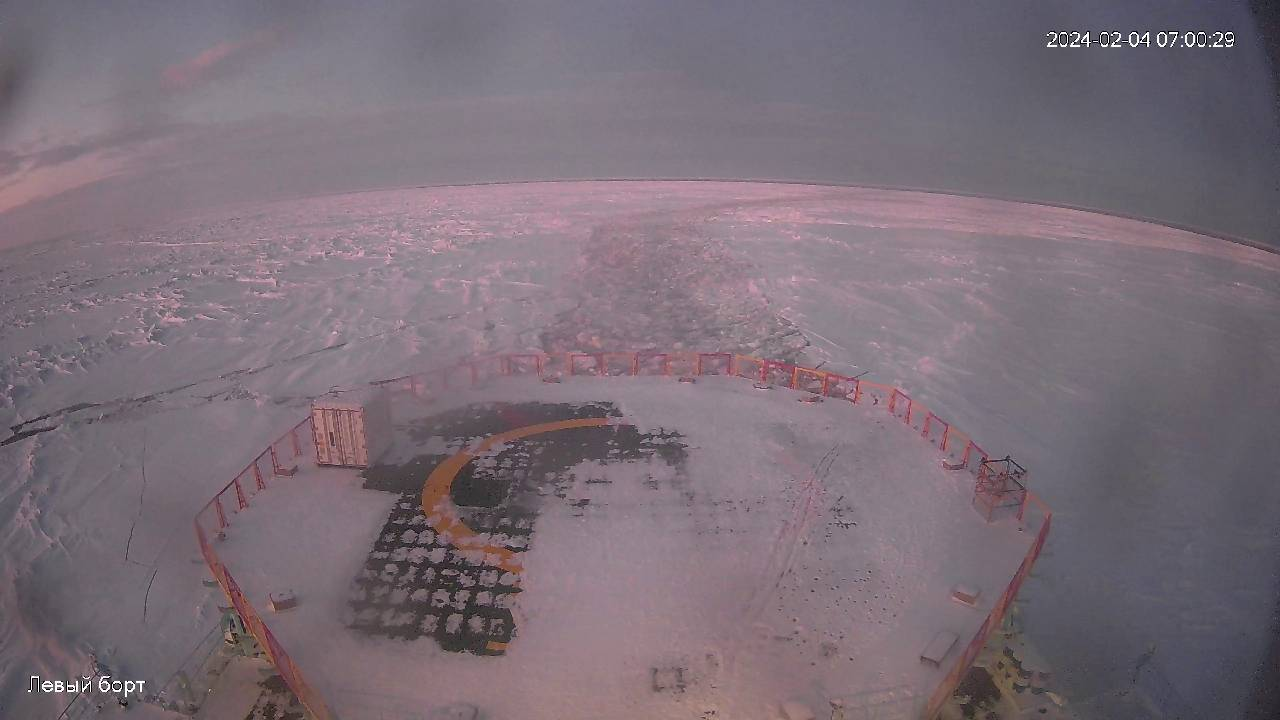
\includegraphics[scale=0.18]{src/Project_planning/assets/6513.jpg}}
    \subfloat[Канал, покрытый ледяным салом]{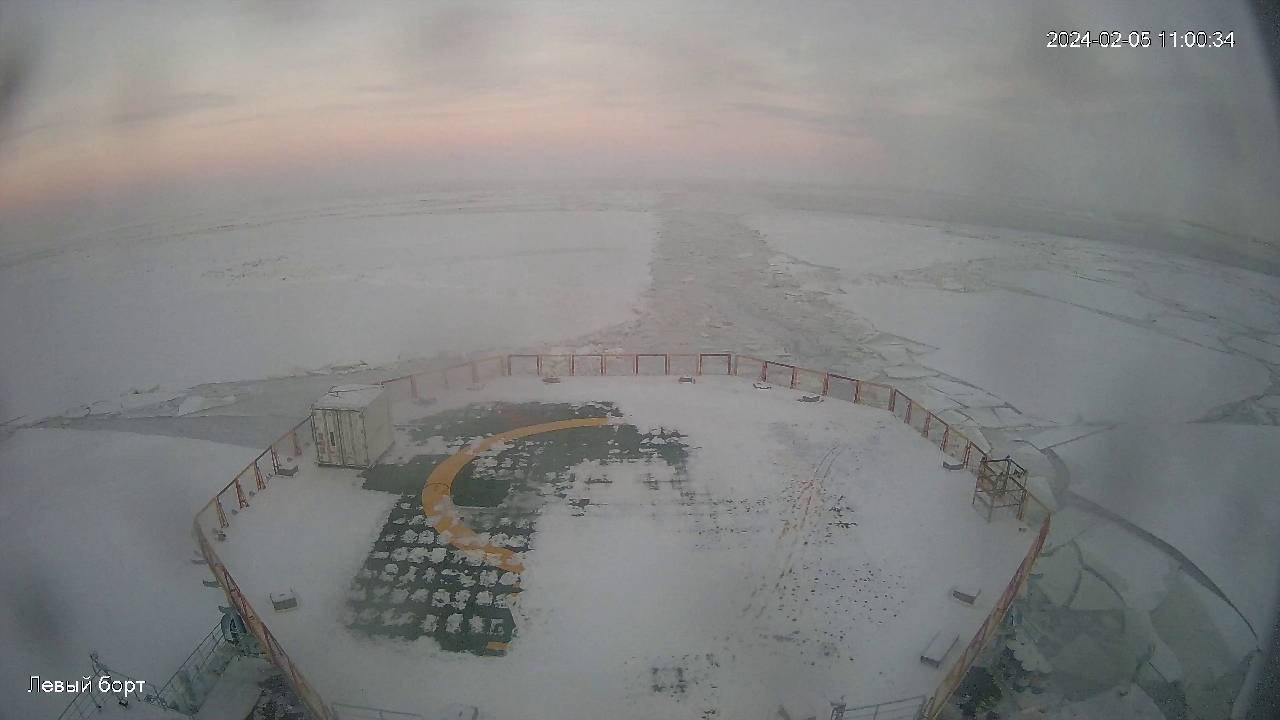
\includegraphics[scale=0.18]{src/Project_planning/assets/Заросший канал.jpg}}
    \caption{Сравнение кадров канала}\label{fig:closed channel}
\end{figure}
Оба описанных выше подхода также имеют некоторые общие ограничения.
\begin{enumerate}
    \item Отсутствие размеченных датасетов. Сейчас компьютерное зрение особенно сильно развивается в сфере автомобилей с автопилотом, в то время как для более специфических тем наработок немного. 
    Так как данный проект является первым в России (и, возможно, в мире), который ставит перед собой задачу анализа ледовой обстановки, 
    то не было возможности использовать какие-либо наработки в этой области в виду их отсутствия (по крайней мере в открытом доступе). В первую очередь это касается размеченных датасетов. 
    Это отразилось на методах, которые использовались во время работы.
    \item Сложность выделения ледового канала. Эта проблема отчасти связана с предыдущей. Выделять ледовый канал даже человеку порой бывает трудно, из-за чего результаты
    работы алгоритмов могут быть шумными, а также их оценка представляет собой нетривиальную задачу. На Рис.~\ref{fig:closed channel} представлены примеры канала. 
    Канал \textbf{a} уже зарос, в то время как канал \textbf{b} просто покрыт ледяным салом.
\end{enumerate} 


\section{Анализ литературы}
\subsection{Введение}
Поскольку задача была разбита на два этапа, то и анализ литературы производился в два этапа:
\begin{enumerate}
    \item Методы сегментации, не использующие глубокое обучение
    \item Методы сегментации, использующие глубокое обучение
\end{enumerate}

Однако оба анализа ставили целью найти подходы, использующие алгоритмы без размеченных датасетов.

\subsection{Методы сегментации, не использующие глубокое обучение}
Для сегментации изображений без использования глубокого обучения было решено обратить внимание на классические методы кластеризации, 
такие как KMeans\cite{kmeans}, DBSCAN\cite{dbscan} и EM\cite{em1} алгоритмы, поскольку сегментация в данном подходе будет в основном зависеть от цвета пикселей.

После проведенных экспериментов было решено остановится на EM алгоритме. DBSCAN не представлялось возможным использовать из-за скорости его работы, в то время 
как KMeans не сегментировал изображение так, как это было необходимо.

\subsection{Методы сегментации, использующие глубокое обучение}
Для данного подхода вариативность была куда больше. 
Рассматривались разные подходы к обучению без датасетов, такие как:
\begin{enumerate}
    \item STEGO\cite{stego} данный подход обучает сеть на основе похожести изображений. В сеть подается само изображение, его ближайший сосед и случайное изображение, 
    после чего на основе схожести выходов бэкбоуна данной сети, а также итоговых меток для изображения, его ближайшего соседа и случайного изображения считается лосс, 
    на основе которого и происходит обучение сети. В качестве метрики схожести изображений используется архитектура DINO. Эта статья побудила к использованию DINO в данной работе.
    \item IIC\cite{iic} эта архитектура обучает сеть на основе информационного критерия, сети подаются на вход изображения и их измененные версии. 
    После чего считается информационный критерий и его максимизация является процессом обучения данной архитектуры. Сеть с использованием такого к подхода к обучению 
    была опробована, но, к сожалению, она не дала тех результатов, которые получились в итоге.
    \item DFC\cite{dfc} данный подход напоминает EM алгоритм, который в деталях описан в следующей главе. Идея DFC состоит в том, чтобы выдать метки классов, затем на основе 
    этих псевдометок обновить веса сети, после чего повторить процесс несколько раз. Данный подход также был опробован, но он оказался, во-первых, слишком медленным, а
    во-вторых не выдавал маску того же качества, как реализованный алгоритм 
    \item DINO\cite{DINO} эта архитектура подробно описана в главе ниже, она используется как часть архитектуры итоговой сети.
\end{enumerate}
Некоторые из подходов, описанных выше использовали бэкбоуны (в частности STEGO~\cite{stego}), поэтому было решено исследовать и вопрос обучения бэкбоуна для извлечения 
признаков из изображения. 
\begin{enumerate}
    \item Избавление от шума\cite{denoise}
    \item Решение пазлов\cite{puzzles}
    \item Восстановление части изображения\cite{drawing_backbone}
    \item Предсказание поворота\cite{rotation_prediction}
    \item Использование аугментаций для создания бэкбоуна\cite{augmentations_learning}
\end{enumerate}

\subsection{Итог}
После анализа литературы было принято решение не использовать готовую сеть, а реализовать свою архитектуру. Данное решение продиктовано тем, что рассмотренные подходы
обучались для сегментации и классификации множества различных классов, в то время как сеть для БИК требует возможности сегментации всего на три весьма похожих класса. 
Поэтому рассмотренные выше подходы являлись либо не такими точными, либо избыточными, а в следствие этого тяжелыми с точки зрения вычислений.
Предложенная в этой архитектура нейронной сети представляет собой результат синтеза некоторых идей из упомянутых выше статей и классических подходов в компьютерном зрении.

\section{Методология}
\subsection{Введение}
Как было описано выше, проект был разделен на две части, которые реализовывались отдельно друг от друга, однако они обе имеют общую часть предобработки изображений.

Важно ещё раз отметить, что подход с использованием EM алгоритма разрабатывался в сжатые сроки, являясь временным решением, что, однако, не снимало с него требований 
на точность в детекции канала, хотя это требование не было критическим, т.е. алгоритм мог выдавать шумные маски. 
\subsection{Подход без глубокого обучения}
Для сегментации без использования глубокого обучения использовался EM алгоритм. В него подавалось предобработанное изображение целиком, после чего алгоритм приписывал
каждому пикселю метку класса, основываясь только на цвете пикселя. После чего происходила фильтрация маски (этот процесс описан в конце главы). Данный подход выдавал 
шумные маски, однако даже они позволили начать собирать информацию о ледяном канале в дневное время суток.
\subsubsection{EM алгоритм}
\noindent \textbf{Простой случай}
\\
Предположим есть несколько точек в $d$-мерном пространстве, это наши данные, задача их сегментировать.
\begin{figure}[ht]
    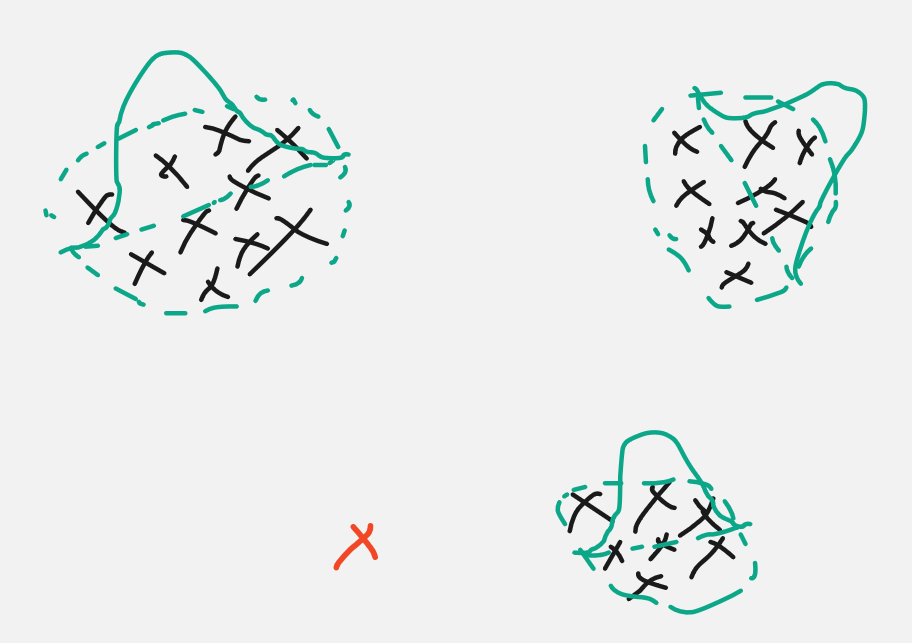
\includegraphics[scale=0.5]{src/Design/assets/em_picture.png}
    \caption{Данные в простом случае}
\end{figure}
Положим, что данные были порождены смесью трёх гауссианов:
\[p(\overline{x}) = \pi_1\cdot p_1(\overline{x}) + \pi_2\cdot p_2(\overline{x}) + \pi_3\cdot p_3(\overline{x}) \]
где
\[\sum\limits_{k=1}^{K} \pi_k = 1 \text{, где } K=3\]
Другими словами, с вероятностью $\pi_i$ будет выбран i-ый гауссиан, после чего будут сгенерированы точки данных на основе этого распределения. 
$\overline{x} \sim p_k(\overline{x})$.
Но возникает вопрос, к какому кластеру отнести новую точку (красную)?
Для этого необходима функция правдоподобия: \\
$\displaystyle p(D|\overline{\theta}) = \prod\limits_{n=1}^N p(\overline{x}_n | \overline{\theta})$ здесь $D$ обозначает весь датасет, другими словами \\$D = \{\overline{x}_n \} _{n=1}^N$
\\
Где
\[p(\overline{x} | \overline{\theta}) = \sum\pi_k\cdotp_k(\overline{x}) = \sum\limits_{k}\pi_k\cdot\mathcal{N}(\overline{x}|\overline{\mu}_k, \Sigma_k)\]
Где $\overline{\mu}_i \text{ и } \Sigma_i$ --- параметры плотности нормального распределения, а

\[\overline{\theta} = (\pi_1, \dots \pi_K,
\overline{\mu}_1, \Sigma_1, \dots, \overline{\mu}_K, \Sigma_K)\] 
После чего:
\[p(D|\overline{\theta}) = \prod\limits_{n=1}^N p(\overline{x}_n | \overline{\theta}) =
 \prod\limits_{n=1}^N (\pi_1\cdot p_1(\overline{x}_n | \overline{\theta}_1) + \pi_2\cdot p_2(\overline{x}_n | \overline{\theta}_2) + 
 \dots + \pi_K\cdot p_K(\overline{x}_n | \overline{\theta}_K) ) \overset{}{\underset{\overline{\theta}}{\rightarrow}} \text{max}\]
 Где $\overline{\theta}_i = (\overline{\mu}_i, \Sigma_i)$
\\
Проблема в том, что это произведение большого числа сумм, из-за чего это сложно максимизировать
Идея в том, чтобы посмотреть на распределение, правдоподобие и порождающий процесс и понять, какая еще информация об этом процессе необходима, чтобы
облегчить максимизацию правдоподобия.
\\
Оказывается, что добавление к $\overline{x}$ меток класса сильно облегчает максимизацию. В математическом виде это можно представить так:

\[ Z = \{\overline{z}_n \} _{n=1}^N \text{, где каждый } \overline{z}_n \text{ в one-hot представлении: } \overline{z}_n = (0,\dots,1,\dots0)\] 
% and only 1 of this vector is on the kth position, which means that $x_n \in C_k$, where $C_k$ means cluster number k.
% So if $Z$ is known, then
Поэтому если $Z$ известно, то
\[p(D, Z | \overline{\theta}) = \prod\limits_{n=1}^{N}p(\overline{x}_n, \overline{z}_n | \overline{\theta})
= \prod\limits_{n=1}^{N}p(\overline{z}_n | \overline{\pi})\cdot p(\overline{x}_n| \overline{z}_n, \overline{\theta})
= \prod\limits_{n=1}^{N}\prod\limits_{k=1}^{K}{(\pi_k\cdot\mathcal{N}(\overline{x}_n|\overline{\mu}_k,\Sigma_k))}^{{z_n}_k}\]

\[\log(p(D, Z | \overline{\theta})) = \sum\limits_{n=1}^{N}\sum\limits_{k=1}^{K}{z_n}_k \cdot (\log(\pi_k) +  \log(\mathcal{N}(\overline{x}_n|\overline{\mu}_k,\Sigma_k)))\]
\[= \sum\limits_{k=1}^K \log(\pi_k) \cdot \sum\limits_{n=1}^N {z_n}_k + 
\sum\limits_{k=1}^K \big( \sum\limits_{n=1}^N {z_n}_k \cdot \log(\mathcal{N}(\overline{x}_n|\overline{\mu}_k,\Sigma_k)) \big)\]
Можно заметить, что первое и второе слагаемые зависят от разных параметров.
Первое слагаемое зависит от $\pi_k$, а второе от параметров плотности нормального распределения $\overline{\mu}_k, \Sigma_k$. Это даёт возможность максимизировать слагаемые независимо.
\\
И главная идея в следующем. Сложная функция правдоподобия становится простой, если известны скрытые параметры ($Z$). 
Поэтому процесс максимизации можно разбить на два шага 
\begin{enumerate}
    \item E-шаг (зафиксировать $\overline{\theta}$, найти $\mathbb{E}[Z]$):
    \[\mathbb{E}[z_{n, k}] = p(C_k|\overline{x}_n,\overline{\theta}) 
    = \displaystyle \frac{p(C_k|\overline{\theta})\cdot p(\overline{x}_n|C_k,\overline{\theta})}{\sum\limits_{l=1}^K p(C_l|\overline{\theta})\cdot p(\overline{x}_n|C_l,\overline{\theta})}
    = \displaystyle \frac{\pi_k\cdot \mathcal{N}(\bar x_n | \bar \mu_k, \Sigma_k)}{\sum\limits_{l=1}^K \pi_l \cdot \mathcal{N}(\bar x_n | \bar \mu_l, \Sigma_l)}\]
    \item M-шаг (зафиксировать $\mathbb{E}[Z]$, максимизировать $\mathbb{E}[\log(p(D,Z|\overline{\theta}))]$). В большинстве случаев вместо $Z$, можно использовать его мягкие оценки $\mathbb{E}(Z)$:
    \[\mathbb{E}[\log p(D,Z|\bar\theta)] 
    = \mathbb{E}\Big[\sum\limits_n\sum\limits_k {z_n}_k \cdot \big(\log(p(\overline{x}_n|\overline{\mu}_k, \Sigma_k)) + \log(\pi_k)\big)\Big]\] 
    \[ = \sum\limits_n\sum\limits_k\mathbb{E}[{z_n}_k]\cdot(\log(\pi_k) + \log\big(p(\overline{x}_n|\overline{\mu}_k, \Sigma_k)))\]
    \[= \sum\limits_k\Big(\sum\limits_n\mathbb{E}[z_{n,k}]\Big) \log \pi_k + \sum\limits_k\sum\limits_n\mathbb{E}[z_{n,k}]\cdot \log p(\bar x_n|\bar\mu_k,\Sigma_k)\]
\end{enumerate}

\noindent\textbf{Общий случай}
\\
Даны:
\begin{enumerate}
    \item X \- датасет
    \item Z \- скрытые параметры (они неизвестны)
    \item $\theta$ \- параметры модели, которые тоже неизвестны
\end{enumerate}
Задача --- максимизировать $p(X|\theta)$, что является сложной задачей, однако максимизация $p(X, Z|\theta)$ сильно легче. Поэтому пусть
\[Q(\theta, \theta^{(n)}) := \mathbb{E}_{p(Z|X,\theta^{(n)})} \big[\log p(X,Z|\theta)\big]
= \int \log p(X,Z|\theta) \cdot p(Z|X,\theta^{(n)}) dz \]
И на каждой итерации:
\[\theta^{(n+1)} = \underset{\theta}{\mathrm{argmax }}\text{ } Q(\theta, \theta^{(n)})\]
\\
Итерации продолжаются до тех пор пока $\theta$ или правдоподобие не перестанут меняться (теоретически это должно произойти одновременно). 
Также стоит отметить, что правдоподобие должно только увеличиваться после каждой итерации. Поэтому имеем:
\[\log(p(X|\theta)) > \log(p(X|\theta^{(n)}))\]
\[\log(p(X|\theta)) - \log(p(X|\theta^{(n)})) 
= \log \Big( \int p(X,Z|\theta) dz \Big) - \log(p(X|\theta^{(n)})) \]
\[= \log \Big(\int p(Z|X,\theta^{(n)} \cdot \displaystyle \frac{p(X,Z|\theta)}{p(Z|X,\theta^{(n)})}) dz \Big) - \log(p(X|\theta^{(n)}))\]
\[= \log\Big( \mathbb{E}_{p(Z|X,\theta^{(n)})}\big[\displaystyle\frac{p(X,Z|\theta)}{p(Z|X,\theta^{(n)})} \big] \Big) - \log(p(X|\theta^{(n)})) \]
\[ \underset{\text{по неравенству Йенсена}}{\geq} \mathbb{E}_{p(Z|X,\theta^{(n)})}\Big[\log\big(\displaystyle\frac{p(X,Z|\theta)}{p(Z|X,\theta^{(n)})} \big) \Big]  - \log(p(X|\theta^{(n)})) \]
\[ = \mathbb{E}_{p(Z|X,\theta^{(n)})}\Big[\log\big(\displaystyle\frac{p(X,Z|\theta)}{p(Z|X,\theta^{(n)}) \cdot p(X|\theta^{(n)})} \big) \Big]\]
Важно заметить, что $p(Z|X,\theta^{(n)}) \cdot p(X|\theta^{(n)}) = p(X,Z|\theta^{(n)})$

\noindent И поэтому:
\[ \log(p(X|\theta)) \geq \log(p(X|\theta^{(n)})) + \mathbb{E}_{p(Z|X,\theta^{(n)})}\Big[\log\big(\displaystyle\frac{p(X,Z|\theta)}{p(Z|X,\theta^{(n)}) \cdot p(X|\theta^{(n)})} \big) \Big] =: \mathcal{L}(\theta, \theta^{(n)})\]

\begin{figure}[h]
    \begin{center}
        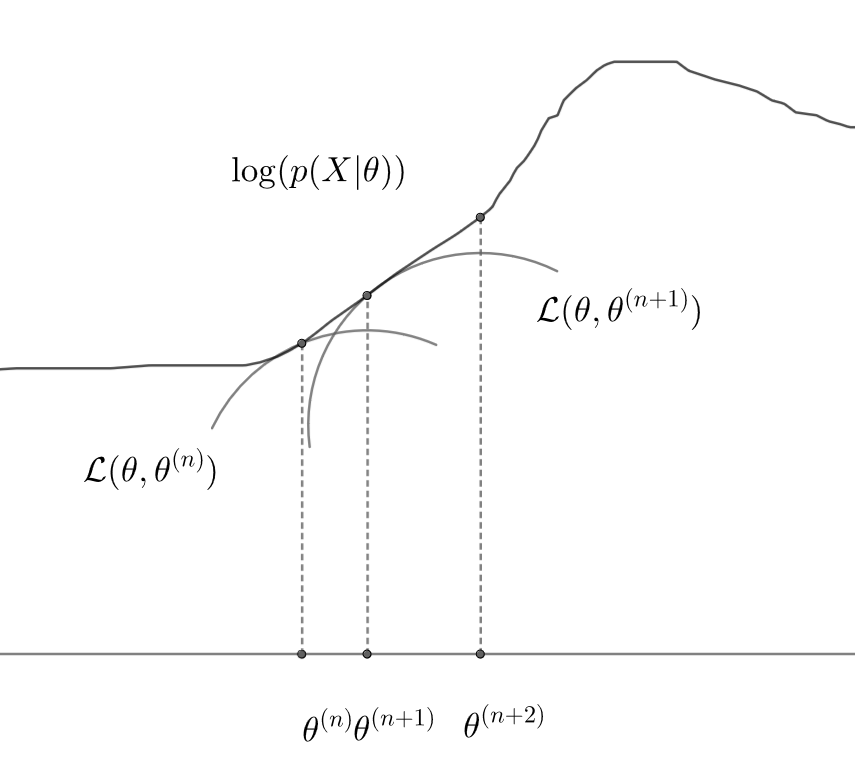
\includegraphics[scale=0.45]{src/Design/assets/em_visualisation.png}
    \end{center}
    \caption{Визуализация алгоритма}\label{fig:em_visual}
\end{figure}

\noindent Как показано на Рис.~\ref{fig:em_visual}, в каждой точке  ($\theta^{(n)}$, $\theta^{(n+1)}$, $\theta^{(n+2)}$ и т.д.) известно наименьшее значение $\log(p(X|\theta))$, при этом оно же равно $\mathcal{L}(\theta, \theta^{(n)})$
\\
Также важно заметить, что $\log(p(X|\theta^{(n)})) = \mathcal{L}(\theta^{(n)}, \theta^{(n)})$
\\
Поэтому идея --- оптимизировать $\mathcal{L}(\theta, \theta^{(n)})$. Эта функция сходится к локальному максимуму, что тоже неплохо.
\\
Однако в начале было указано, что необходимо оптимизировать $Q(\theta, \theta^{(n)})$, но оказывается, что оптимизация $Q$ и $\mathcal{L}$ --- это одна и та же задача.
\\
\[ \mathcal{L}(\theta, \theta^{(n)}) = \underset{const(\theta)}{\log(p(X|\theta^{(n)}))} + \underset{\text{это и есть } Q(\theta, \theta^{(n)})}{\mathbb{E}_{p(Z|X,\theta^{(n)})}\Big[\log\big(p(X,Z|\theta) \big) \Big]}\]
\[- \underset{const(\theta)}{\mathbb{E}_{p(Z|X,\theta^{(n)})}\Big[\log\big(p(X,Z|\theta^{(n)})\big)\Big]}
    \]

\subsection{Подход с глубоким обучением}
Во втором подходе использовалась следующая архитектура (на Рис~\ref{nn_architecure}):
\begin{enumerate}
    \item Бэкбоун --- сверточная четырехслойная сеть
    \item DINO --- трансформер для извлечения дополнительных фич
    \item Классификатор --- свертка $1\times 1$ с тремя выходными каналами
\end{enumerate}
\begin{figure}[h]
    \begin{center}
        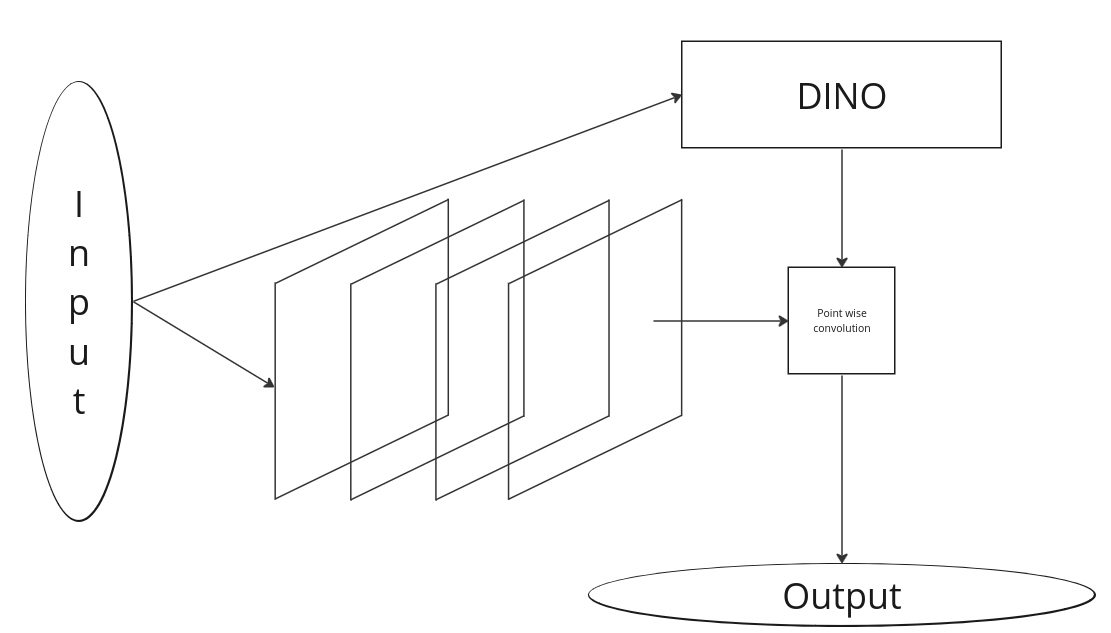
\includegraphics[scale=0.4]{src/Design/assets/NN_architecure.png}
    \end{center}
    \caption{Архитектура нейросети}\label{nn_architecure}
\end{figure}
Было решено создать небольшой датасет и сделать обучение с учителем, предварительно обучив бэкбоун и используя DINO для получения дополнительных признаков 
по всему изображению.
\subsubsection{Бэкбоун}
Бэкбоун обучался на классической задаче решения пазлов, т.е. в бэкбоун подавались части изображения, а на выход ожидался один из четырех классов, 
показывающих расположение части фотографии. Данный подход позволил бэкбоуну научиться извлекать признаки, характерные для изображений датасета, что позволило получить 
относительно неплохие результаты, о которых речь пойдет в следующей главе. В качестве основного блока бэкбоуна использовался стандартный блок из:
\begin{enumerate}
    \item Свертка $3\times 3$
    \item Батч нормализация
    \item ReLU
    \item Дропаут слой
\end{enumerate}

\subsubsection{DINO}
\noindent\textbf{Предпосылки к использованию DINO} \\
DINO --- это архитектура Visual Transformer (ViT) и подход к его обучению. Данная архитектура хорошо себя показывает в извлечении признаков, на основе которых 
можно находить ближайших соседей изображений, что показано в статье про архитектуру STEGO~\cite{stego}. Поэтому было решено включить DINO в итоговую архитектуру, чтобы
улучшить качество сегментации.
\\
\textbf{Архитектура DINO} \\
Основная идея сети --- предсказание выхода учителя, построенного с помощью кодировщика с моментом, используя кросс-энтропию в качестве лосс функции.
\\
В основе DINO лежит архитектура Vision Transformer (ViT), которая обучается без учителя. В DINO используются две сети: ученик и учитель. 
Ученик обновляется на каждом шаге градиента, в то время как веса учителя обновляются с помощью скользящего среднего весов ученика.
\\
Самообучение в DINO происходит следующим образом.
На вход каждой сети подаётся изображение $x$, на выход сети выдают $K$-мерный вектор $P$ с вероятностями (полученный при помощи softmax с температурой):
\[P_s{(x)}^{(i)} = \frac{\exp(g_{\theta_s}{(x)}^{(i)} / \tau_s)}{\sum\limits_{k=1}^K\exp(g_{\theta_s}{(x)}^{(k)} / \tau_s)}\]
\\
Здесь $\tau_s$ --- температура, контролирующая ``остроту'' выхода. Для сети-учителя применяется такое же преобразование.
\\
Далее, учительская сеть замораживается, а сеть-ученик обучается с использованием кросс-энтропии и идеи ``локально-глобального соответствия''. Для этого 
из каждой фотографии входного батча составляется набор искаженных кропов (вырезов или обрезанных частей) изображения $V$. 
При этом в этом наборе содержатся два ``глобальных кропа'' изображения (покрывающих более 50\% изображения): $x_1, x_2$; и несколько локальных кропов. 
Все кропы подаются в сеть-ученик, а в сеть-учитель только глобальные кропы. Затем для обучения сети-ученика минимизируется следующий лосс:
\[\overset{}{\underset{\theta_s}{\min}} \sum\limits_{x\in\{x_1,x_2\}} \sum\limits_{x'\in V; x' \neq x}H(P_t(x), P_s(x'))\]
Где $H(a,b) = -a\cdot\log(b)$
\\
Для обновления весов учительской сети используется следующий подход (важно отметить, что сеть-учитель и сеть-ученик отличаются только весами, 
архитектуры у них одинаковые):
\[\theta_t \leftarrow \lambda \theta_t + (1-\lambda)\cdot \theta_s\]
Где $\lambda$ изменяется по ``косинусному расписанию'' (cosine scheduling) от $0.996$ до $1$.
\\
\noindent Также важно отметить, что многие архитектуры обучения без учителя подвержены вырожденым решениям (когда все кластеризуется в один кластер), чтобы этого не случилось в 
DINO используется центрирование и ``заострение'' при помощи температуры, описанное выше. Эти две техники имеют противоположные эффекты, 
что даёт возможность избежать вырожденного решения. Центрирование смещает сеть ближе к равномерному распределению, в то время как ``заострение'' противодействует этому.
Центрирование можно рассматривать, как смещение (bias) в сети, однако оно обновляется используя экспоненциально скользящее среднее. что кстати нивелирует 
зависимость от размера батча:
\[c\leftarrow mc + (1-m)\frac{1}{B}\sum\limits_{i=1}^B g_{\theta_t}(x_i)\]
\\
Здесь $B$ --- размер батча, а $m$ --- параметр, влияющий на скорость обновления параметра $c$.
\\  
Примерный код обучения DINO представлен в листинге~1~\cite{DINO}


\begin{lstlisting}[label=algo1, language=Python, float=tp, caption={Алгоритм обучения DINO}]
# gs, gt: student and teacher networks
# C: center (K)
# tps, tpt: student and teacher temperatures
# l, m: network and center momentum rates
gt.params = gs.params
for x in loader: # load a minibatch x with n samples
    x1, x2 = augment(x), augment(x) # random views
    s1, s2 = gs(x1), gs(x2) # student output n-by-K
    t1, t2 = gt(x1), gt(x2) # teacher output n-by-K
    loss = H(t1, s2)/2 + H(t2, s1)/2
    loss.backward() # back-propagate
    # student, teacher and center updates
    update(gs) # SGD
    gt.params = l*gt.params + (1-l)*gs.params
    C = m*C + (1-m)*cat([t1, t2]).mean(dim=0)
def H(t, s):
    t = t.detach() # stop gradient
    s = softmax(s / tps, dim=1)
    t = softmax((t - C) / tpt, dim=1) # center + sharpen
    return - (t * log(s)).sum(dim=1).mean()
\end{lstlisting}

\subsubsection{Итоговая сеть}
Как было указано в начале подглавы итоговая сеть в качестве головы имеет свертку $1\times1$. Для обучения этой головы, был размечен небольшой 
датасет на 100 изображений, 80 из которых использовались для обучения, 20 для валидации результата. В качестве лосс функции использовалась стандартная кросс-энтропия:

\[L(x,y) = -w_y \cdot \log\frac{\exp(x_y)}{\sum\limits_{c=1}^C \exp(x_c)}\]
Здесь, $x$ --- выход нейросети, $y$ --- ground-truth метка, а $w$ --- веса для каждого класса. В обучении использовались следующие веса: 10 для воды и ледяного сала, 1 для воды.
В итоговой сети использовался уже предобученный DINO, что позволило увеличить целевые метрики.

\subsubsection{Фильтрация выхода}
Поскольку нейросеть обучалась на небольшом датасете, а многие изображения трудно различимы, то не все ответы нейросети используются. Вместо этого в течение определенного 
небольшого времени алгоритм работает, накапливая результаты, после чего выбирается результат, являющийся медианой всех полученных данных, и именно он считается 
результатом работы алгоритма. В качестве значения, по которому находится медиана, используется ширина канала, которая определяется на основе полученной маски.

Данный подход используется, дабы уменьшить влияние шума и артефактов изображения.

\subsection{Предобработка изображений}

\begin{figure}[htbp]
    \centering
    \subfloat[Изначальное изображение]{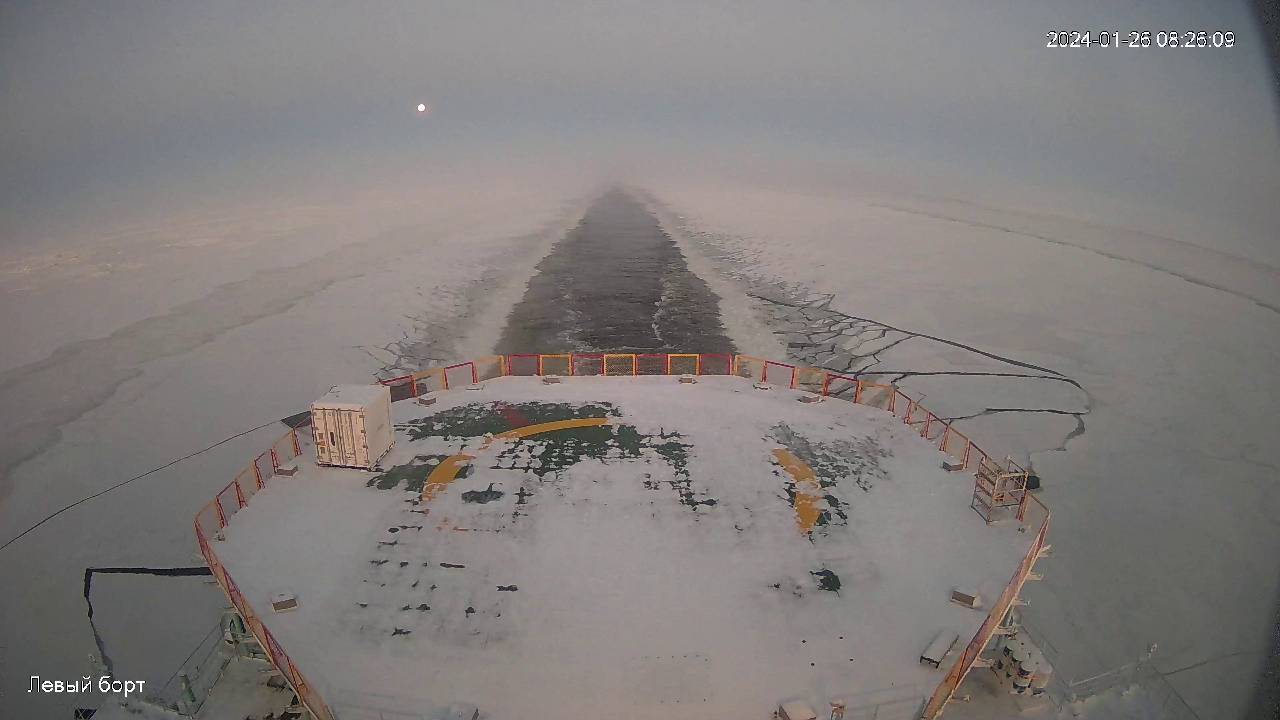
\includegraphics[scale=0.18]{src/Design/assets/raw.png}}
    \subfloat[Компенсация рыбьего глаза]{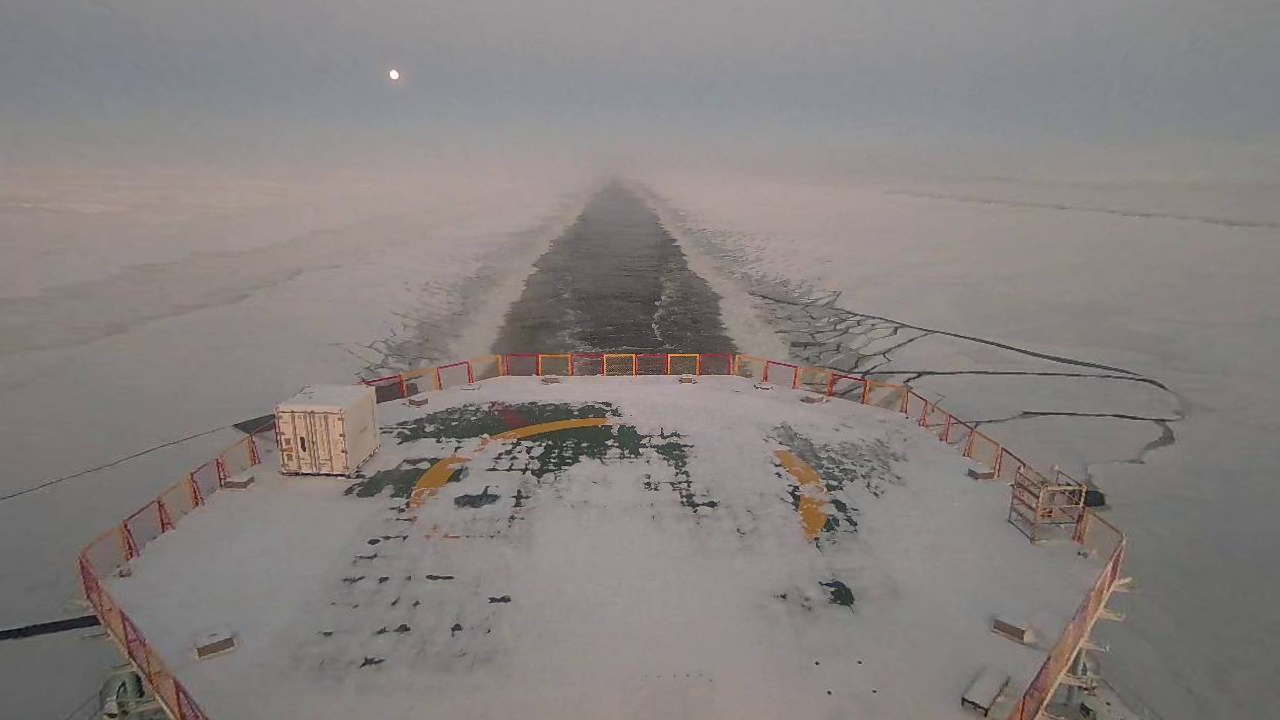
\includegraphics[scale=0.18]{src/Design/assets/undistored.png}}
    \\
    \subfloat[Обрезание по вертикали]{
\includegraphics[scale=0.18]{src/Design/assets/vertical_cropped.png}}
    \subfloat[Повышение контрастности]{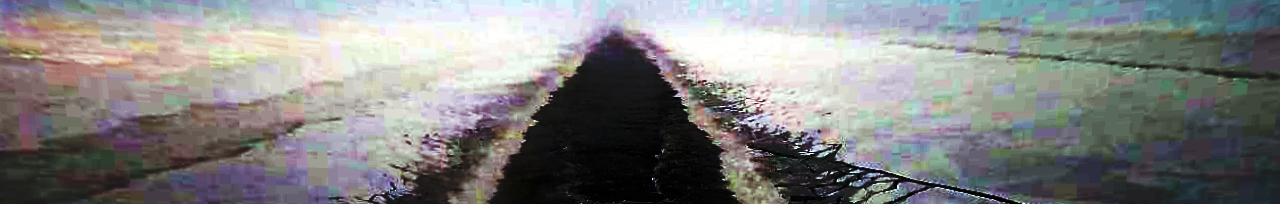
\includegraphics[scale=0.18]{src/Design/assets/equalised.png}}
    \\
    \subfloat[Обрезание по горизонтали]{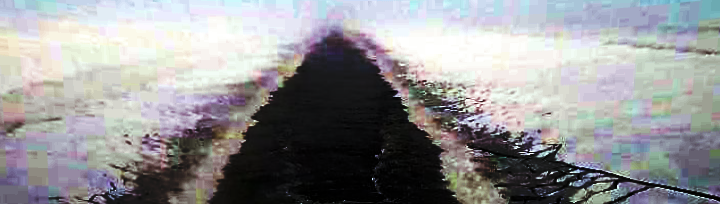
\includegraphics[scale=0.2]{src/Design/assets/horizontal_cropped.png}}
    \caption{Предобработка изображения}\label{fig:preprocessing}
\end{figure}

Этап предобработки изображений одинаков для EM алгоритма и нейросети. Сначала в изображении компенсируется рыбий глаз, вызванный камерой, далее изображение обрезается 
по вертикали. Так как камера установлена статично, то на изображении всегда на одинаковых позиция присутствует как часть кормы судна, так и часть неба. Оба этих 
элемента не имеют отношения к сегментации канала, они, напротив, добавляют сложности к задачи сегментации, поскольку EM алгоритм больше выделяет части судна в 
отдельный кластер, а бэкбоун нейросети больше обучается на признаках судна, нежели на текстуре канала. Исходя из этих наблюдений было решено обрезать эту часть 
изображения. Далее у изображения повышается контрастность, путем выравнивания гистограммы и обрезаются края по горизонтали, так как при повышении контрастности 
они становятся темнее, чем центральная часть изображения, что приводит к неверной сегментации. Такое изображение подается в ЕМ и нейросеть. 

\begin{figure}[htbp]
    \centering
    \subfloat[Маска EM алгоритма]{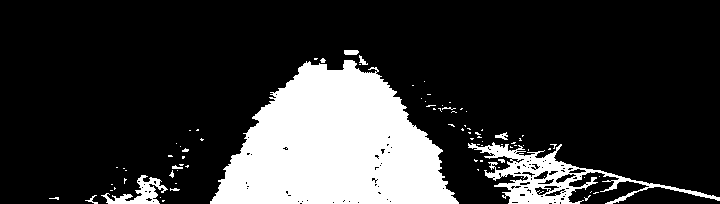
\includegraphics[scale=0.2]{src/Design/assets/em_mask.png}}
    \subfloat[Применение эрозивной фильтрации]{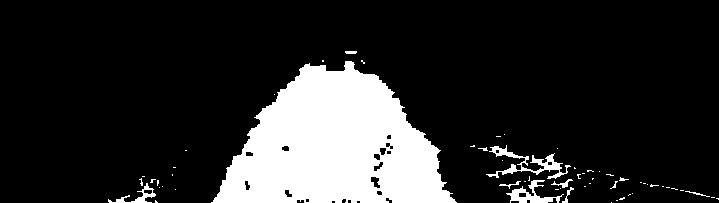
\includegraphics[scale=0.2]{src/Design/assets/morf_mask.png}}
    \\
    \subfloat[Применение BFS для окончательной фильтрации]{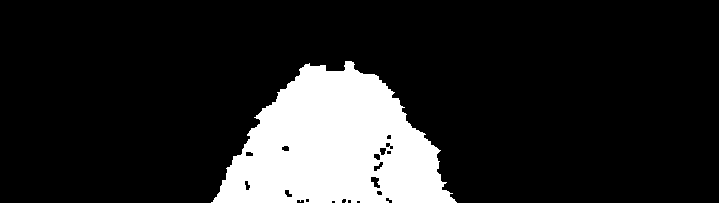
\includegraphics[scale=0.2]{src/Design/assets/bfs_mask.png}}
    \caption{Постобработка маски ЕМ алгоритма}\label{fig:postprocessing}
\end{figure}

В случае ЕМ алгоритма был реализован небольшой постпроцессинг, так как маска, выдаваемая EM алгоритмом, довольно шумная. В первую очередь происходит эрозивная 
фильтрация, чтобы немного избавиться от шума и отделить маску канала от неправильно классифицированных пикселей, после чего применяется поиск в графе. Начальными 
``вершинами'' считаются пиксели, лежащие по центру кадра (там всегда начинается канал), затем в маску добавляются все пиксели отмеченные, как принадлежащие каналу, 
которые являются соседними с уже добавленными в маску. Такой подход позволяет отделить канал от неправильных меток по бокам изображения, которые возникают из-за
изменения яркости картинки после повышения контрастности, что было описано выше.

На Рис.~\ref{fig:preprocessing} приведены этапы предобработки изображений для обоих подходов, а на Рис.~\ref{fig:postprocessing} постобработки 
масок EM алгоритма
\include{src/Implementation/Implementation}
\section{Результаты}
В данной главе представлены результаты применения разработанного метода сегментации ледового канала с использованием нейросети. 
На маске, являющейся выходом нейросети, присутствуют три класса: вода, ледяное сало и лёд. Вода в объединении с ледяным салом 
формируют канал. Несмотря на определенные достижения, итоговый подход оказался неидеальным. Далее приведены основные метрики качества полученных результатов.

\subsection{Метрики}

Для оценки эффективности работы нейросети были использованы метрики полнота (recall) и точность (precision) для каждого класса отдельно, а также для канала в целом. 
\[Recall = \frac{TP}{TP + FN}; Precision = \frac{TP}{TP + FP}\]
Здесь $TP$ --- истинно положительный результат, $FN$ --- ложно отрицательный, $FP$ --- ложно положительный. Полнота позволяет понять долю правильно классифицированных 
пикселей из всех пикселей данного класса, в то время как точность отвечает за долю правильно классифицированных пикселей из всех пикселей, 
классифицированных в данный класс.
Результаты оценки приведены в Таблице~\ref{tab:nn_results}.
\begin{table}[h]
    \centering 
        \begin{tabular}{|c|c|c|} 
            \hline
            & Полнота & Точность \\
            \hline
            Вода & 0.64 & 0.47 \\ \hline
            Ледяное сало & 0.48 & 0.51 \\ \hline
            Канал & 0.86 & 0.61 \\ \hline
        \end{tabular}
    \caption{Качество маски}\label{tab:nn_results}
\end{table}

Из таблицы видно, что Recall для воды составил 0.64, а Precision — 0.47, что указывает на относительно высокую способность модели обнаруживать воду, 
но при этом значительное количество ложно положительных срабатываний. Аналогично, для ледяного сала метрики составили 0.48 и 0.51 соответственно, что также 
указывает на неполное соответствие предсказаний и истинных значений.

Однако не смотря на низкие метрики у каждого класса по отдельности, канал в целом выделяется удачно, хотя и с большим количеством ложных классификаций. Это достигается 
тем, что нейросеть иногда классифицирует воду, как ледяное сало и наоборот, что негативно сказывается на метриках этих классов, но никак не влияет на метрику канала в целом.

\subsection{Пример маски}

Для демонстрации полученных результатов на Рис.~\ref{fig:nn_mask} представлен пример маски канала, полученной в ходе сегментации.

\begin{figure}[htbp]
    \centering
    \subfloat[Изначальное изображение]{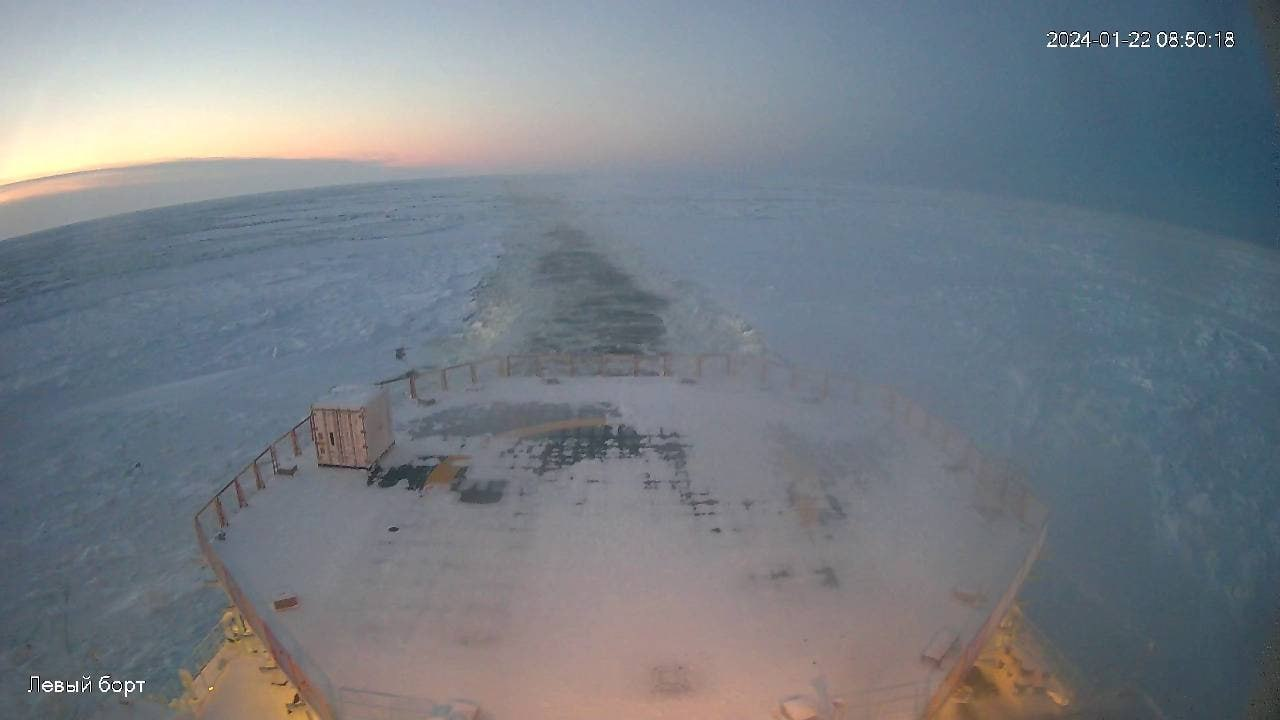
\includegraphics[scale=0.2]{src/Testing/assets/raw.jpg}}
    \subfloat[Маска нейросети]{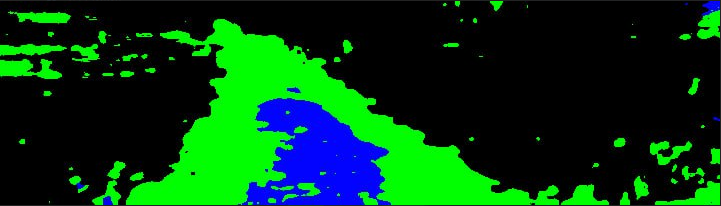
\includegraphics[scale=0.2]{src/Testing/assets/mask.png}}
    \\
    \caption{Результат работы нейросети}\label{fig:nn_mask}
\end{figure}

Здесь отображены области, отнесенные к трём классам: вода (синий цвет), ледяное сало (зелёный цвет) и лёд (чёрный цвет). 
Объединение синих и зеленых областей формирует сегментированный канал. Как видно из примера, нейросеть успешно выявляет основные контуры канала, 
однако присутствуют некоторые неточности и ложноположительные области.

\subsection{Итог}

Результаты сегментации показали, что разработанный метод способен достаточно эффективно выявлять ледовый канал позади ледокола. 
Высокий Recall канала (0.86) свидетельствует о том, что метод корректно идентифицирует большинство участков канала. 
Однако, относительно низкий Precision (0.61) указывает на наличие ложных положительных определений.

В целом, предложенный метод сегментации продемонстрировал свою применимость для выделения ледового канала, но он требует дополнительной фильтрации результатов, 
которая описана в главе выше.

\section{Заключение}

В данной дипломной работе было описано решение задачи по выделению ледового канала на изображении с кормы ледокола, с использованием подходов с глубоким обучением и без него.
Главной задачей проекта было разработка алгоритма, способного выделить пиксельную маску ледового канала для упрощения его дальнейшего исследования и нахождения его 
характеристик, таких как ширина или скорость схождения.

В ходе выполнения проекта были разобраны современные методы сегментации изображений, был проведен анализ существующих решений в области глубокого обучения без учителя, 
а также рассмотрены классические (без глубокого обучения) подходы к сегментации. Анализ существующих подходов именно в этой сфере, помог нивелировать проблему отсутствия
размеченных датасетов арктических льдов и позволил провести обучение нейросети на относительно небольшом датасете.

Для решения задачи было реализовано два подхода: подход без глубокого обучения, чтобы установить его на судно до конца декабря 2023 года, чтобы уже плавающий ледокол мог собирать 
какие-то данные, второй подход использовал нейросеть для более точного обнаружения канала и установки на ледокол после его прибытия в порт. Оба подхода способны генерировать пиксельные маски канала. 
Проведенное тестирование сети показало, что предложенный метод способен эффективно выделять ледовый канал, однако результаты оказались не идеальными. 
Основными проблемами стали появление шумов и неточностей в маске, что связано с разнообразием условий съемки и сложностью ледовых структур.

Даже с текущими неточностями и ограничениями нейросетевой подход может и будет использован на практике. Он позволяет автоматизировать сбор и первичный анализ информации
о ледовом канале, облегчая работу команде ледокола. В дальнейшем планируется дорабатывать существующий алгоритм, как программно, улучшая нейросеть, так и технически, 
добавляя новые типы сенсоров.

Таким образом, результаты данной работы демонстрируют перспективность использования нейросетевых методов для сегментации ледового канала. Продолжение 
исследований в этом направлении, включая сбор более разнообразных данных и улучшение архитектуры модели, может привести к созданию более надежных и 
точных инструментов для навигации в арктических водах. Данный алгоритм в составе БИК будет установлен летом 2024 года на 4 ледокола серии Урал и на ледокол ``50 лет победы''.

\bibliographystyle{ieeetr} % We choose the "plain" reference style
\bibliography{refs} % Entries are in the refs.bib file
\end{document}